% This is samplepaper.tex, a sample chapter demonstrating the
% LLNCS macro package for Springer Computer Science proceedings;
% Version 2.20 of 2017/10/04
%
\documentclass[runningheads]{llncs}
% 
\usepackage{graphicx}
% Used for displaying a sample figure. If possible, figure files should
% be included in EPS format.
%
% If you use the hyperref package, please uncomment the following line
% to display URLs in blue roman font according to Springer's eBook style:
% \renewcommand\UrlFont{\color{blue}\rmfamily}

\begin{document}
%
\title{Contribution Title\thanks{Supported by organization x.}}
%
% \titlerunning{Abbreviated paper title}
% If the paper title is too long for the running head, you can set
% an abbreviated paper title here
%
\author{Diogo Esteves\inst{1} \and
Rui Sousa\inst{1}}
%
\authorrunning{F. Author et al.}
% First names are abbreviated in the running head.
% If there are more than two authors, 'et al.' is used.
%
\institute{Department of Informatics, University of Minho, Portugal
\ \url{http://www.di.uminho.pt} }%
\maketitle              % typeset the header of the contribution
%
\begin{abstract}
The abstract should briefly summarize the contents of the paper in
15--250 words.

\keywords{First keyword  \and Second keyword \and Another keyword.}
\end{abstract}
%
%
%
\section{Introduction}
In contemporary society, the intersection of poverty, obesity prevalence, and mental illness represents a complex web of interconnected health and socioeconomic challenges. While access to food is often viewed as a basic human necessity, the quality and nutritional value of available food sources significantly impact individual health outcomes. Contrary to the conventional notion that poverty equates to a lack of food, impoverished communities frequently grapple with limited access to nutritious options, leading to a reliance on heavily processed, calorie-dense foods. This dietary pattern not only exacerbates the prevalence of obesity but also contributes to a host of associated health complications, including diabetes and cardiovascular diseases.

Furthermore, the ramifications of poor dietary habits extend beyond physical health, exerting profound effects on mental well-being. Mounting evidence suggests a bidirectional relationship between obesity and mental illness, with each condition influencing and exacerbating the other. As individuals navigate the challenges of poverty, the stressors associated with financial instability and limited resources often compound existing mental health vulnerabilities, predisposing them to conditions such as depression and anxiety.

Against this backdrop, this study aims to confirm the interplay between poverty, obesity, and mental illness through a comprehensive analysis of prevalence data by analysing the prevalence rates of these phenomena across diverse socioeconomic strata. 

Specifically, we seek to elucidate whether a relationship exists wherein the prevalence of obesity escalates with ascending levels of poverty and to explore the intricate relationship between obesity, poverty, and mental health outcomes.

\paragraph Estado da arte – Revisão da literatura existente sobre o mesmo tema ou temas semelhantes. 
Discussão de trabalhos anteriores e lacunas identificadas.

\section{Materials and data sources}


\paragraph{Dataset sources} 

The datasets that are used throughout this investigative work are sourced from the Our World in Data repository. We have selected three specific datasets from three different studies, each studying the incidence and prevalence of extreme poverty, obesity and mental illnesses throughout the years. 

\paragraph{Dataset on Obesity} 

The dataset on obesity studies a myriad of factors related to obesity and their respective correlation, from comparing prevalence in men vs women, risk of coronary diseases, death rate, etcetera. For the purpose of this study we will be solely focusing on the data related to the prevalence of obesity in adults / share of adults who are overweight or obese.

\paragraph{Dataset on Poverty} 

The dataset on poverty by its turn measures a wide array of aspects related to poverty, from an inequality point of view. The dataset contains data regarding the levels of poverty and daily budgets, impacts from world scale events (e.g. COVID-19 pandemic), among others. For the purpose of this study we will be solely using the data corresponding to number in poverty considering an extreme poverty threshold of USD 2.15 / day in global income / consumption.

\paragraph{Dataset on Mental Health} 

Similarly to the aforementioned datasets the dataset on mental illnesses analyses the prevalence, burden of disease and risk factors of several mental illnesses globally, however we will be solely focusing on the prevalence of mental disorders namely depressive, bipolar and anxiety disorders, schizophrenia. The dataset also contains data on eating disorders which we will also attempt to correlate with data on obesity.

To further enrich the available data we have also sourced a global population throughout the years dataset from Our World in Data. [referencias] The datasets

obesidade - https://ourworldindata.org/obesity#all-charts
mental - https://ourworldindata.org/mental-health
pobreza - https://ourworldindata.org/poverty
population - https://ourworldindata.org/population-growth

Ver como citar


\section{Methods}



\paragraph Métodos – Explicação da arquitetura implementada bem como da função de cada um dos seus componentes. 



\paragraph

Numa primeira abordagem visamos estudar o impacto da pobreza na obesidade e saúde mental. Em causa estará, por exemplo, a redução do acesso a alimentação saudável (podemos também introduzir um dataset de preço de alimentos por exemplo) e de que forma a falta de recursos possivelmente possa induzir stress/depressão.




\subsubsection{Sample Heading (Third Level)} Only two levels of
headings should be numbered. Lower level headings remain unnumbered;
they are formatted as run-in headings.

\paragraph{Sample Heading (Fourth Level)}
The contribution should contain no more than four levels of
headings. Table~\ref{tab1} gives a summary of all heading levels.

\begin{table}
\caption{Table captions should be placed above the
tables.}\label{tab1}
\begin{tabular}{|l|l|l|}
\hline
Heading level &  Example & Font size and style\\
\hline
Title (centered) &  {\Large\bfseries Lecture Notes} & 14 point, bold\\
1st-level heading &  {\large\bfseries 1 Introduction} & 12 point, bold\\
2nd-level heading & {\bfseries 2.1 Printing Area} & 10 point, bold\\
3rd-level heading & {\bfseries Run-in Heading in Bold.} Text follows & 10 point, bold\\
4th-level heading & {\itshape Lowest Level Heading.} Text follows & 10 point, italic\\
\hline
\end{tabular}
\end{table}


\noindent Displayed equations are centered and set on a separate
line.
\begin{equation}
x + y = z
\end{equation}
Please try to avoid rasterized images for line-art diagrams and
schemas. Whenever possible, use vector graphics instead (see
Fig.~\ref{fig1}).

\begin{figure}
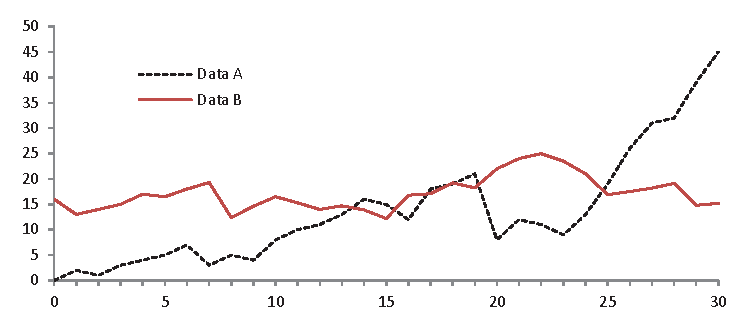
\includegraphics[width=\textwidth]{fig1.eps}
\caption{A figure caption is always placed below the illustration.
Please note that short captions are centered, while long ones are
justified by the macro package automatically.} \label{fig1}
\end{figure}

\begin{theorem}
This is a sample theorem. The run-in heading is set in bold, while
the following text appears in italics. Definitions, lemmas,
propositions, and corollaries are styled the same way.
\end{theorem}
%
% the environments 'definition', 'lemma', 'proposition', 'corollary',
% 'remark', and 'example' are defined in the LLNCS documentclass as well.
%
\begin{proof}
Proofs, examples, and remarks have the initial word in italics,
while the following text appears in normal font.
\end{proof}
For citations of references, we prefer the use of square brackets
and consecutive numbers. Citations using labels or the author/year
convention are also acceptable. The following bibliography provides
a sample reference list with entries for journal
articles~\cite{ref_article1}, an LNCS chapter~\cite{ref_lncs1}, a
book~\cite{ref_book1}, proceedings without editors~\cite{ref_proc1},
and a homepage~\cite{ref_url1}. Multiple citations are grouped
\cite{ref_article1,ref_lncs1,ref_book1},
\cite{ref_article1,ref_book1,ref_proc1,ref_url1}.
%
% ---- Bibliography ----
%
% BibTeX users should specify bibliography style 'splncs04'.
% References will then be sorted and formatted in the correct style.
%
% \bibliographystyle{splncs04}
% \bibliography{mybibliography}
%
\begin{thebibliography}{8}
\bibitem{ref_article1}
Author, F.: Article title. Journal \textbf{2}(5), 99--110 (2016)

\bibitem{ref_lncs1}
Author, F., Author, S.: Title of a proceedings paper. In: Editor,
F., Editor, S. (eds.) CONFERENCE 2016, LNCS, vol. 9999, pp. 1--13.
Springer, Heidelberg (2016). \doi{10.10007/1234567890}

\bibitem{ref_book1}
Author, F., Author, S., Author, T.: Book title. 2nd edn. Publisher,
Location (1999)

\bibitem{ref_proc1}
Author, A.-B.: Contribution title. In: 9th International Proceedings
on Proceedings, pp. 1--2. Publisher, Location (2010)

\bibitem{ref_url1}
LNCS Homepage, \url{http://www.springer.com/lncs}. Last accessed 4
Oct 2017
\end{thebibliography}
\end{document}
